\documentclass{standalone}
\usepackage{tikz}
\usetikzlibrary{shapes.geometric, arrows}


\definecolor{mycolor}{RGB}{0, 153, 255}
\tikzstyle{process} = [rectangle, rounded corners,
                       minimum width=2cm, minimum height=1cm,
                       text centered, draw=black, fill=mycolor,
                       text=white, line width=0.3mm]

\tikzstyle{arrow} = [thick,->,>=stealth]

\begin{document}
    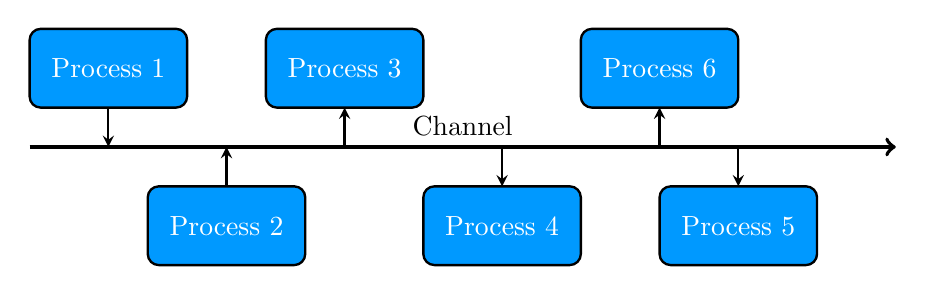
\begin{tikzpicture}[node distance=2cm]
        
        \draw [->, line width=0.5mm] (-1, 0) -- node[anchor=south] {Channel} (10, 0);
        
        
        
        \node (Process1) [process, xshift=0cm, yshift=1cm] {Process 1};
        
        \node (Process2) [process, xshift=1.5cm, yshift=-1cm] {Process 2};
        
        \node (Process3) [process, xshift=3cm, yshift=1cm] {Process 3};
        
        \node (Process4) [process, xshift=5cm, yshift=-1cm] {Process 4};
        
        \node (Process5) [process, xshift=8cm, yshift=-1cm] {Process 5};
        
        \node (Process6) [process, xshift=7cm, yshift=1cm] {Process 6};
        
        
        \draw [arrow] (0,0.5) -- (0, 0); %process 1
        \draw [arrow] (1.5,-0.5) -- (1.5, 0); %process 2
        \draw [arrow] (3,0) -- (3, 0.5); %process 3
        \draw [arrow] (5,0) -- (5, -0.5); %process 4
        \draw [arrow] (8,0) -- (8, -0.5); %process 5
        \draw [arrow] (7,0) -- (7, 0.5); %process 6
        
        
        
    
    \end{tikzpicture}
\end{document}
